% Options for packages loaded elsewhere
\PassOptionsToPackage{unicode}{hyperref}
\PassOptionsToPackage{hyphens}{url}
%
\documentclass[
  letterpaper,
  oneside,
  open=any]{scrbook}

\usepackage{amsmath,amssymb}
\usepackage{iftex}
\ifPDFTeX
  \usepackage[T1]{fontenc}
  \usepackage[utf8]{inputenc}
  \usepackage{textcomp} % provide euro and other symbols
\else % if luatex or xetex
  \usepackage{unicode-math}
  \defaultfontfeatures{Scale=MatchLowercase}
  \defaultfontfeatures[\rmfamily]{Ligatures=TeX,Scale=1}
\fi
\usepackage{lmodern}
\ifPDFTeX\else  
    % xetex/luatex font selection
\fi
% Use upquote if available, for straight quotes in verbatim environments
\IfFileExists{upquote.sty}{\usepackage{upquote}}{}
\IfFileExists{microtype.sty}{% use microtype if available
  \usepackage[]{microtype}
  \UseMicrotypeSet[protrusion]{basicmath} % disable protrusion for tt fonts
}{}
\makeatletter
\@ifundefined{KOMAClassName}{% if non-KOMA class
  \IfFileExists{parskip.sty}{%
    \usepackage{parskip}
  }{% else
    \setlength{\parindent}{0pt}
    \setlength{\parskip}{6pt plus 2pt minus 1pt}}
}{% if KOMA class
  \KOMAoptions{parskip=half}}
\makeatother
\usepackage{xcolor}
\setlength{\emergencystretch}{3em} % prevent overfull lines
\setcounter{secnumdepth}{5}
% Make \paragraph and \subparagraph free-standing
\ifx\paragraph\undefined\else
  \let\oldparagraph\paragraph
  \renewcommand{\paragraph}[1]{\oldparagraph{#1}\mbox{}}
\fi
\ifx\subparagraph\undefined\else
  \let\oldsubparagraph\subparagraph
  \renewcommand{\subparagraph}[1]{\oldsubparagraph{#1}\mbox{}}
\fi

\providecommand{\tightlist}{%
  \setlength{\itemsep}{0pt}\setlength{\parskip}{0pt}}\usepackage{longtable,booktabs,array}
\usepackage{calc} % for calculating minipage widths
% Correct order of tables after \paragraph or \subparagraph
\usepackage{etoolbox}
\makeatletter
\patchcmd\longtable{\par}{\if@noskipsec\mbox{}\fi\par}{}{}
\makeatother
% Allow footnotes in longtable head/foot
\IfFileExists{footnotehyper.sty}{\usepackage{footnotehyper}}{\usepackage{footnote}}
\makesavenoteenv{longtable}
\usepackage{graphicx}
\makeatletter
\def\maxwidth{\ifdim\Gin@nat@width>\linewidth\linewidth\else\Gin@nat@width\fi}
\def\maxheight{\ifdim\Gin@nat@height>\textheight\textheight\else\Gin@nat@height\fi}
\makeatother
% Scale images if necessary, so that they will not overflow the page
% margins by default, and it is still possible to overwrite the defaults
% using explicit options in \includegraphics[width, height, ...]{}
\setkeys{Gin}{width=\maxwidth,height=\maxheight,keepaspectratio}
% Set default figure placement to htbp
\makeatletter
\def\fps@figure{htbp}
\makeatother
% definitions for citeproc citations
\NewDocumentCommand\citeproctext{}{}
\NewDocumentCommand\citeproc{mm}{%
  \begingroup\def\citeproctext{#2}\cite{#1}\endgroup}
\makeatletter
 % allow citations to break across lines
 \let\@cite@ofmt\@firstofone
 % avoid brackets around text for \cite:
 \def\@biblabel#1{}
 \def\@cite#1#2{{#1\if@tempswa , #2\fi}}
\makeatother
\newlength{\cslhangindent}
\setlength{\cslhangindent}{1.5em}
\newlength{\csllabelwidth}
\setlength{\csllabelwidth}{3em}
\newenvironment{CSLReferences}[2] % #1 hanging-indent, #2 entry-spacing
 {\begin{list}{}{%
  \setlength{\itemindent}{0pt}
  \setlength{\leftmargin}{0pt}
  \setlength{\parsep}{0pt}
  % turn on hanging indent if param 1 is 1
  \ifodd #1
   \setlength{\leftmargin}{\cslhangindent}
   \setlength{\itemindent}{-1\cslhangindent}
  \fi
  % set entry spacing
  \setlength{\itemsep}{#2\baselineskip}}}
 {\end{list}}
\usepackage{calc}
\newcommand{\CSLBlock}[1]{\hfill\break#1\hfill\break}
\newcommand{\CSLLeftMargin}[1]{\parbox[t]{\csllabelwidth}{\strut#1\strut}}
\newcommand{\CSLRightInline}[1]{\parbox[t]{\linewidth - \csllabelwidth}{\strut#1\strut}}
\newcommand{\CSLIndent}[1]{\hspace{\cslhangindent}#1}

\usepackage[default]{opensans}
\fontseries{lc}\selectfont
\definecolor{nmfsblue1}{HTML}{00467f}
\definecolor{nmfsblue2}{HTML}{007eb2}
\makeatletter
\@ifpackageloaded{bookmark}{}{\usepackage{bookmark}}
\makeatother
\makeatletter
\@ifpackageloaded{caption}{}{\usepackage{caption}}
\AtBeginDocument{%
\ifdefined\contentsname
  \renewcommand*\contentsname{Table of contents}
\else
  \newcommand\contentsname{Table of contents}
\fi
\ifdefined\listfigurename
  \renewcommand*\listfigurename{List of Figures}
\else
  \newcommand\listfigurename{List of Figures}
\fi
\ifdefined\listtablename
  \renewcommand*\listtablename{List of Tables}
\else
  \newcommand\listtablename{List of Tables}
\fi
\ifdefined\figurename
  \renewcommand*\figurename{Figure}
\else
  \newcommand\figurename{Figure}
\fi
\ifdefined\tablename
  \renewcommand*\tablename{Table}
\else
  \newcommand\tablename{Table}
\fi
}
\@ifpackageloaded{float}{}{\usepackage{float}}
\floatstyle{ruled}
\@ifundefined{c@chapter}{\newfloat{codelisting}{h}{lop}}{\newfloat{codelisting}{h}{lop}[chapter]}
\floatname{codelisting}{Listing}
\newcommand*\listoflistings{\listof{codelisting}{List of Listings}}
\makeatother
\makeatletter
\makeatother
\makeatletter
\@ifpackageloaded{caption}{}{\usepackage{caption}}
\@ifpackageloaded{subcaption}{}{\usepackage{subcaption}}
\makeatother

\usepackage{hyphenat}
\usepackage{ifthen}
\usepackage{calc}
\usepackage{calculator}

\usepackage{graphicx}
\usepackage{wallpaper}

\usepackage{geometry}

\usepackage{graphicx}
\usepackage{geometry}
\usepackage{afterpage}
\usepackage{tikz}
\usetikzlibrary{calc}
\usetikzlibrary{fadings}
\usepackage[pagecolor=none]{pagecolor}


% Set the titlepage font families







% Set the coverpage font families

\ifLuaTeX
  \usepackage{selnolig}  % disable illegal ligatures
\fi
\IfFileExists{bookmark.sty}{\usepackage{bookmark}}{\usepackage{hyperref}}
\IfFileExists{xurl.sty}{\usepackage{xurl}}{} % add URL line breaks if available
\urlstyle{same} % disable monospaced font for URLs
\hypersetup{
  pdftitle={An example tech memo},
  pdfauthor={Jane Doe; Eva Nováková; Matti Meikäläinen; Ashok Kumar},
  hidelinks,
  pdfcreator={LaTeX via pandoc}}

\title{An example tech memo}
\usepackage{etoolbox}
\makeatletter
\providecommand{\subtitle}[1]{% add subtitle to \maketitle
  \apptocmd{\@title}{\par {\large #1 \par}}{}{}
}
\makeatother
\subtitle{The subtitle}
\author{Jane Doe \and Eva Nováková \and Matti Meikäläinen \and Ashok
Kumar}
\date{2023-01-01}

\begin{document}
%%%%% begin titlepage extension code

  \begin{frontmatter}

\begin{titlepage}
% This is a combination of Pandoc templating and LaTeX
% Pandoc templating https://pandoc.org/MANUAL.html#templates
% See the README for help

\thispagestyle{empty}

\newgeometry{top=-100in}

% Page color

\newcommand{\coverauthorstyle}[1]{{\fontsize{20}{24.0}\selectfont
#1}}

\begin{tikzpicture}[remember picture, overlay, inner sep=0pt, outer sep=0pt]

\tikzfading[name=fadeout, inner color=transparent!0,outer color=transparent!100]
\tikzfading[name=fadein, inner color=transparent!100,outer color=transparent!0]
\node[anchor=south west, rotate=0.0, opacity=1.0] at ($(current page.south west)+(0pt, 8.75in)$) {

\includegraphics[width=\paperwidth, keepaspectratio]{images/cover-header-2.png}};

% Title
\newcommand{\titlelocationleft}{2.3in}
\newcommand{\titlelocationbottom}{7in}
\newcommand{\titlealign}{left}

\begin{scope}{%
\fontsize{50}{60.0}\selectfont
\node[anchor=north
west, align=left, rotate=0] (Title1) at ($(current page.south west)+(\titlelocationleft,\titlelocationbottom)$)  [text width = 5in]  {\textcolor{nmfsblue1}{\nohyphens{An
example tech memo}}};
}
\end{scope}

% Author
\newcommand{\authorlocationleft}{2.3in}
\newcommand{\authorlocationbottom}{5in}
\newcommand{\authoralign}{left}

\begin{scope}
{%
\fontsize{20}{24.0}\selectfont
\node[anchor=north
west, align=left, rotate=0] (Author1) at ($(current page.south west)+(\authorlocationleft,\authorlocationbottom)$)  [text width = 5in]  {
\coverauthorstyle{Jane Doe, Eva Nováková, Matti Meikäläinen, Ashok
Kumar\\}};
}
\end{scope}

% Header
\newcommand{\headerlocationleft}{2.3in}
\newcommand{\headerlocationbottom}{9.8in}
\newcommand{\headerlocationalign}{left}

\begin{scope}
{%
\fontsize{16}{19.2}\selectfont
 \node[anchor=north west, align=left, rotate=0] (Header1) at %
($(current page.south west)+(\headerlocationleft,\headerlocationbottom)$)  [text width = 5in]  {\textcolor{white}{\nohyphens{NOAA
Technical Memorandum NMFS-XXX-\#\#}}};
}
\end{scope}

% Footer
\newcommand{\footerlocationleft}{6in}
\newcommand{\footerlocationbottom}{0.1\paperheight}
\newcommand{\footerlocationalign}{left}

\begin{scope}
{%
\fontsize{8}{9.6}\selectfont
 \node[anchor=north west, align=left, rotate=0] (Footer1) at %
($(current page.south west)+(\footerlocationleft,\footerlocationbottom)$)  [text width = 2.5in]  {{\nohyphens{U.S.
DEPARTMENT OF COMMERCE\\
\strut \\
National Oceanic and Atmospheric Administration\\
National Marine Fisheries Service\\
Northwest Fisheries Science Center}}};
}
\end{scope}

% Date
\newcommand{\datelocationleft}{6in}
\newcommand{\datelocationbottom}{2in}
\newcommand{\datelocationalign}{left}

\begin{scope}
{%
\fontsize{20}{24.0}\selectfont
 \node[anchor=north west, align=left, rotate=0] (Date1) at %
($(current page.south west)+(\datelocationleft,\datelocationbottom)$)  [text width = 2.5in]  {{\nohyphens{January
2023}}};
}
\end{scope}

\end{tikzpicture}
\clearpage
\restoregeometry
%%% TITLE PAGE START

% Set up alignment commands
%Page
\newcommand{\titlepagepagealign}{
\ifthenelse{\equal{left}{right}}{\raggedleft}{}
\ifthenelse{\equal{left}{center}}{\centering}{}
\ifthenelse{\equal{left}{left}}{\raggedright}{}
}
%% Titles
\newcommand{\titlepagetitlealign}{
\ifthenelse{\equal{left}{right}}{\raggedleft}{}
\ifthenelse{\equal{left}{center}}{\centering}{}
\ifthenelse{\equal{left}{left}}{\raggedright}{}
\ifthenelse{\equal{left}{spread}}{\makebox[\linewidth][s]}{}
}


\newcommand{\titleandsubtitle}{
% Title and subtitle
{\fontsize{30}{36.0}\selectfont
\textcolor{nmfsblue1}{\bfseries{\nohyphens{An example tech memo}}}\par
}%

\vspace{\betweentitlesubtitle}
{
{\textit{\nohyphens{The subtitle}}}\par
}}
\newcommand{\titlepagetitleblock}{
\titleandsubtitle
}

\newcommand{\authorstyle}[1]{{\fontsize{20}{24.0}\selectfont
#1}}

\newcommand{\affiliationstyle}[1]{{#1}}

\newcommand{\titlepageauthorblock}{
{\authorstyle{\nohyphens{Jane
Doe}{\textsuperscript{1}}\textsuperscript{,}{\textsuperscript{2}},  \nohyphens{Eva
Nováková}{\textsuperscript{2}},  \nohyphens{Matti
Meikäläinen}{\textsuperscript{3}}\textsuperscript{,}{\textsuperscript{*}} and \nohyphens{Ashok
Kumar}{\textsuperscript{4}}\textsuperscript{,}{\textsuperscript{5}}}}}

\newcommand{\titlepageaffiliationblock}{
\hangindent=1em
\hangafter=1
{\affiliationstyle{
{1}.~Northwest Fisheries Science Center,~Conservation Biology
Division,~2725 Montlake Boulevard EastSeattle, Washington 98112
\par\hangindent=1em\hangafter=1{2}.~University of Washington,~School of
Aquatic and Fisheries Sciences
\par\hangindent=1em\hangafter=1{3}.~University of Kemijärvi,~Department
of Biological and Environmental Science,~Kylmäniementie 79, 98120,
KEMIJÄRVI, Finland
\par\hangindent=1em\hangafter=1{4}.~University of Minnesota,~Department
of Mathematics
\par\hangindent=1em\hangafter=1{5}.~HØnefoss Institute,~R Tradição 35,
Portugal 2950-726


\vspace{1\baselineskip} 
* \textit{Correspondence:}~Matti Meikäläinen~matti@jy.fi
}}
}
\newcommand{\headerstyled}{%
{}
}
\newcommand{\footerstyled}{%
{}
}
\newcommand{\datestyled}{%
{2023-01-01}
}


\newcommand{\titlepageheaderblock}{\headerstyled}

\newcommand{\titlepagefooterblock}{
\footerstyled
}

\newcommand{\titlepagedateblock}{
\datestyled
}

%set up blocks so user can specify order
\newcommand{\titleblock}{\newlength{\betweentitlesubtitle}
\setlength{\betweentitlesubtitle}{1pt}
{\titlepagetitlealign

{\titlepagetitleblock}
}

\vspace{4\baselineskip}
}

\newcommand{\authorblock}{{\titlepageauthorblock}

\vspace{2\baselineskip}
}

\newcommand{\affiliationblock}{{\titlepageaffiliationblock}

\vspace{2\baselineskip}
}

\newcommand{\logoblock}{}

\newcommand{\footerblock}{}

\newcommand{\dateblock}{{\titlepagedateblock}

\vspace{0pt}
}

\newcommand{\headerblock}{}
\newgeometry{top=3in,bottom=1in,right=1in,left=1.75in}
% background image
\newlength{\bgimagesize}
\setlength{\bgimagesize}{0.75\paperwidth}
\LENGTHDIVIDE{\bgimagesize}{\paperwidth}{\theRatio} % from calculator pkg
\ThisULCornerWallPaper{\theRatio}{images/corner-image.png}

\thispagestyle{empty} % no page numbers on titlepages


\newcommand{\vrulecode}{\rule{\vrulewidth}{\textheight}}
\newlength{\vrulewidth}
\setlength{\vrulewidth}{0pt}
\newlength{\B}
\setlength{\B}{\ifdim\vrulewidth > 0pt 0.05\textwidth\else 0pt\fi}
\newlength{\minipagewidth}
\ifthenelse{\equal{left}{left} \OR \equal{left}{right} }
{% True case
\setlength{\minipagewidth}{\textwidth - \vrulewidth - \B - 0.1\textwidth}
}{
\setlength{\minipagewidth}{\textwidth - 2\vrulewidth - 2\B - 0.1\textwidth}
}
\ifthenelse{\equal{left}{left} \OR \equal{left}{leftright}}
{% True case
\raggedleft % needed for the minipage to work
\vrulecode
\hspace{\B}
}{%
\raggedright % else it is right only and width is not 0
}
% [position of box][box height][inner position]{width}
% [s] means stretch out vertically; assuming there is a vfill
\begin{minipage}[b][\textheight][s]{\minipagewidth}
\titlepagepagealign
\headerblock

\titleblock

\authorblock

\affiliationblock

\vfill

\logoblock

\footerblock
\par

\end{minipage}\ifthenelse{\equal{left}{right} \OR \equal{left}{leftright} }{
\hspace{\B}
\vrulecode}{}
\clearpage
\restoregeometry
%%% TITLE PAGE END
\end{titlepage}
\setcounter{page}{1}
\end{frontmatter}

%%%%% end titlepage extension code
\renewcommand*\contentsname{Table of contents}
{
\setcounter{tocdepth}{1}
\tableofcontents
}
\listoffigures
\listoftables
\mainmatter
\bookmarksetup{startatroot}

\chapter*{Citation}\label{citation}
\addcontentsline{toc}{chapter}{Citation}

\markboth{Citation}{Citation}

EE Holmes, 2022. Quarto Report Template. Northwest Fisheries Science
Center.

\bookmarksetup{startatroot}

\chapter{A chapter}\label{a-chapter}

\bookmarksetup{startatroot}

\chapter{Columbia River Chum}\label{columbia-river-chum}

Lorem ipsum dolor sit amet, consectetur adipiscing elit. Clark (1993)
vitae ante quis dui egestas fringilla ac vitae justo (Ansley and Davis
1981; Collins et al. 1996; Deuel and Clark 1968) . Pellentesque quis
magna vel odio malesuada rutrum a volutpat nisl. Aliquam fermentum, urna
eget tristique mattis, augue augue tristique ipsum, eget finibus nunc
eros non nisi. Phasellus mattis hendrerit sapien, quis accumsan dui
pretium eget. Nunc eleifend laoreet urna a luctus. Nulla vel sapien in
nulla gravida tempus sit amet a metus. Vivamus porta condimentum tempus.
Maecenas rhoncus elit id ultricies scelerisque. In gravida urna in
ligula fringilla euismod. Curabitur efficitur porta libero ac fermentum.
Cras fringilla et libero at posuere. Curabitur sodales dapibus elit a
convallis.

Morbi iaculis eget augue eget facilisis. Etiam non orci dignissim,
efficitur purus viverra, pellentesque neque. Aliquam ornare, magna ut
dictum mollis, nunc lorem iaculis nibh, eu consequat lectus urna euismod
tortor. Etiam ut felis nisl. Nunc quis euismod felis. Vestibulum gravida
nisi mi, quis mollis velit ullamcorper non. Aliquam tempus fringilla
bibendum. Lorem ipsum dolor sit amet, consectetur adipiscing elit. Fusce
viverra nulla elementum libero mollis, quis cursus velit sagittis.

\section{General location}\label{general-location}

Morbi iaculis eget augue eget facilisis. Etiam non orci dignissim,
efficitur purus viverra, pellentesque neque. Aliquam ornare, magna ut
dictum mollis, nunc lorem iaculis nibh, eu consequat lectus urna euismod
tortor.

\begin{figure}

\centering{

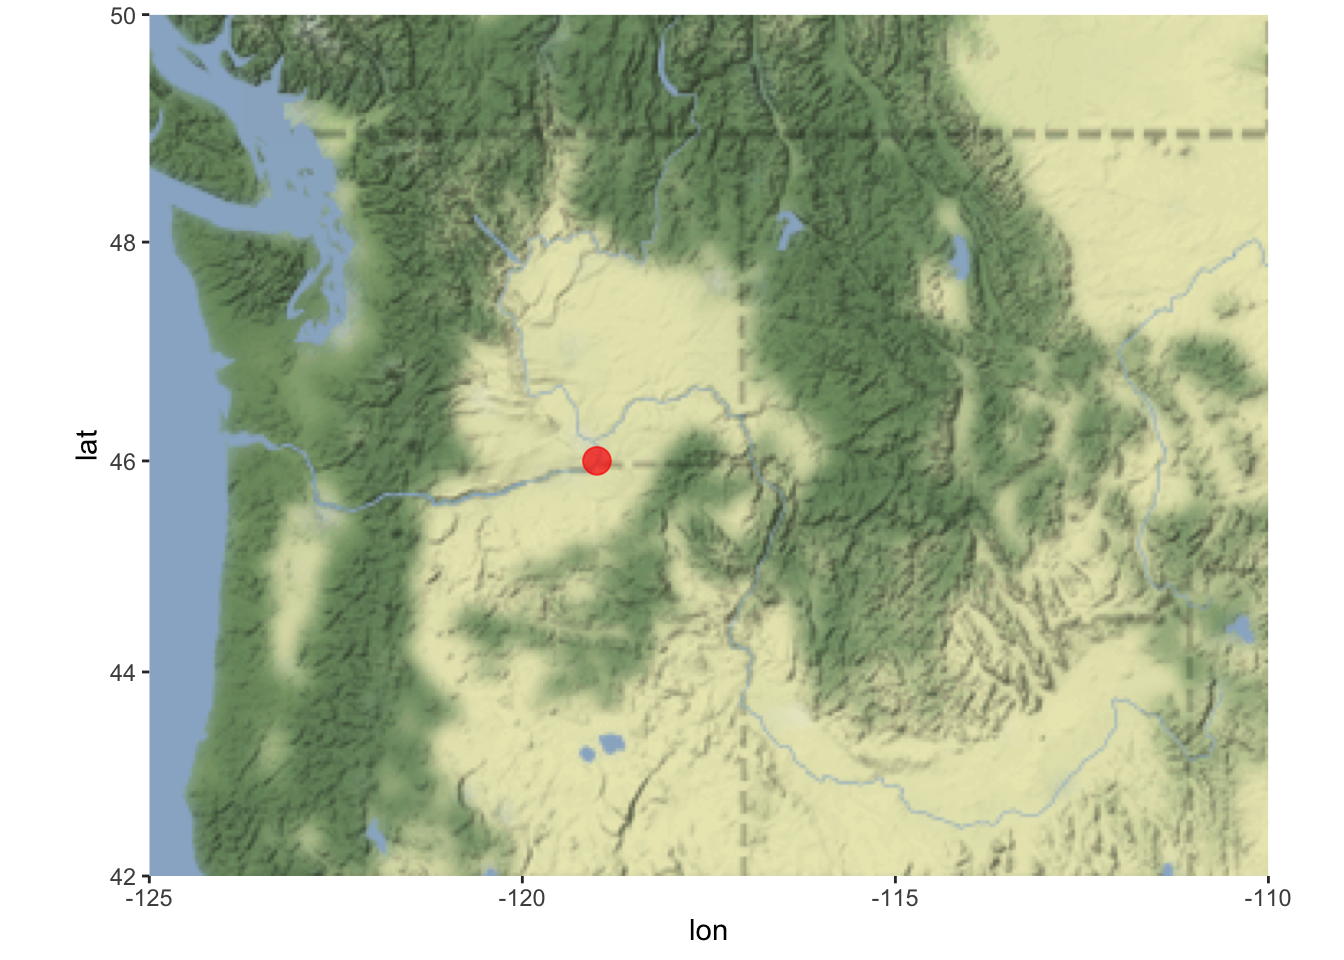
\includegraphics[width=4.48in,height=\textheight]{text/../images/fig-map.png}

}

\caption{\label{fig-map}Morbi iaculis eget augue eget facilisis. Etiam
non orci dignissim, efficitur purus viverra, pellentesque neque. Aliquam
ornare, magna ut dictum mollis.}

\end{figure}%

\section{Recent trends}\label{recent-trends}

Lorem ipsum dolor sit amet, consectetur adipiscing elit. Donec vitae
ante quis dui egestas fringilla ac vitae justo. Pellentesque quis magna
vel odio malesuada rutrum a volutpat nisl. Aliquam fermentum, urna eget
tristique mattis, augue augue tristique ipsum, eget finibus nunc eros
non nisi. Phasellus mattis hendrerit sapien, quis accumsan dui pretium
eget. Nunc eleifend laoreet urna a luctus. Nulla vel sapien in nulla
gravida tempus sit amet a metus. Vivamus porta condimentum tempus.
Maecenas rhoncus elit id ultricies scelerisque. In gravida urna in
ligula fringilla euismod. Curabitur efficitur porta libero ac fermentum.
Cras fringilla et libero at posuere. Curabitur sodales dapibus elit a
convallis.

Morbi iaculis eget augue eget facilisis. Etiam non orci dignissim,
efficitur purus viverra, pellentesque neque. Aliquam ornare, magna ut
dictum mollis, nunc lorem iaculis nibh, eu consequat lectus urna euismod
tortor. Etiam ut felis nisl. Nunc quis euismod felis. Vestibulum gravida
nisi mi, quis mollis velit ullamcorper non. Aliquam tempus fringilla
bibendum. Lorem ipsum dolor sit amet, consectetur adipiscing elit. Fusce
viverra nulla elementum libero mollis, quis cursus velit sagittis.

\begin{figure}

\centering{

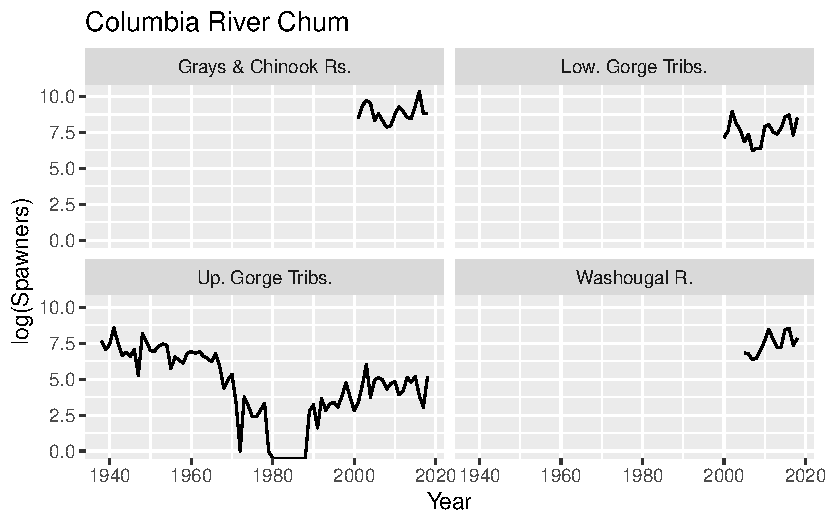
\includegraphics{text/Chapter1_files/figure-pdf/fig-CRchum-status-1.pdf}

}

\caption{\label{fig-CRchum-status}Columbia River Chum. Log spawner count
trends.}

\end{figure}%

\section{Population raw data}\label{population-raw-data}

The raw data can be found in Table~\ref{tbl-CRchum-rawdata}. Nunc quis
euismod felis. Vestibulum gravida nisi mi, quis mollis velit ullamcorper
non. Aliquam tempus fringilla bibendum. Lorem ipsum dolor sit amet,
consectetur adipiscing elit. Fusce viverra nulla elementum libero
mollis, quis cursus velit sagittis.

\begin{table}

\caption{\label{tbl-CRchum-rawdata}Columbia River Chum. Raw Data.}

\centering{

\begin{longtable*}{rr}
\toprule
YEAR & NUMBER\_OF\_SPAWNERS \\ 
\midrule
\multicolumn{2}{l}{Up. Gorge Tribs.} \\ 
\midrule
1990 & 25 \\ 
1991 & 5 \\ 
1992 & 39 \\ 
1993 & 17 \\ 
1994 & 26 \\ 
1995 & 30 \\ 
1996 & 21 \\ 
1997 & 46 \\ 
1998 & 118 \\ 
1999 & 43 \\ 
\midrule
\multicolumn{2}{l}{Low. Gorge Tribs.} \\ 
\midrule
2000 & 1265 \\ 
\midrule
\multicolumn{2}{l}{Grays \& Chinook Rs.} \\ 
\midrule
2001 & 4742 \\ 
2002 & 11713 \\ 
2003 & 16669 \\ 
2004 & 13716 \\ 
2005 & 4204 \\ 
2006 & 6605 \\ 
2007 & 3999 \\ 
2008 & 2608 \\ 
2009 & 2876 \\ 
2010 & 6380 \\ 
2011 & 10809 \\ 
2012 & 8010 \\ 
2013 & 5134 \\ 
2014 & 4792 \\ 
2015 & 11580 \\ 
\bottomrule
\end{longtable*}

}

\end{table}%

\bookmarksetup{startatroot}

\chapter{Conclusion}\label{conclusion}

\section{First off}\label{first-off}

We want to reference the Interior Columbia Upper Columbia Entiat
population Table~\ref{tbl-CRchum-rawdata}. It is in Lorem ipsum dolor
sit amet, consectetur adipiscing elit. Nam commodo sit amet nibh non
molestie. Maecenas hendrerit nisl velit, a condimentum enim lobortis sit
amet. Ut vitae nunc sed mauris condimentum fermentum. Mauris
pellentesque nec neque id elementum. Suspendisse a quam aliquam,
facilisis urna venenatis, malesuada diam. Pellentesque in fringilla
orci. Cras sed purus urna. Ut pharetra enim ut ligula egestas mattis. I
need to reference the work of Hardy (1978).

Phasellus non diam posuere, laoreet velit sed, egestas felis. Etiam eget
neque in tellus lacinia tincidunt. Pellentesque scelerisque odio velit,
nec fringilla nibh iaculis non. Aenean sit amet nulla ipsum. Cras felis
lacus, pulvinar ac nisi et, convallis pulvinar turpis. Morbi non nibh
lacus. Morbi vitae lorem massa. Sed ut turpis vel felis posuere commodo
lacinia ac mi. Donec finibus lectus sit amet elit finibus, vitae rhoncus
ligula tincidunt. Phasellus vitae blandit lacus. Integer sed nisl
fermentum, pulvinar mauris in, posuere enim. Proin sit amet semper urna.
Vivamus aliquet rutrum diam ac luctus.

Quisque in nibh sit amet nunc mollis porttitor quis et mauris. Sed non
condimentum leo, ac condimentum est. Duis ac venenatis nulla, et aliquet
elit. Suspendisse potenti. Duis mollis dui at semper luctus. Maecenas
euismod finibus condimentum. Fusce vitae gravida massa. Mauris metus
est, pretium non semper vel, dictum vel augue.

Curabitur tempus, leo quis volutpat rhoncus, turpis elit vehicula dolor,
id tincidunt augue nunc at enim. In vel enim mattis, varius orci at,
tempus ante. Morbi massa elit, pharetra ac libero at, porta tempus quam.
Ut fringilla, tortor ac tristique euismod, magna felis vestibulum
turpis, quis congue mauris leo nec felis. Aliquam viverra et nibh ut
blandit. Praesent sed luctus odio. Pellentesque finibus velit dolor.
Morbi ac pulvinar ex, id dapibus eros. Cras interdum arcu viverra auctor
tristique. Suspendisse venenatis volutpat ultricies.

Donec bibendum pharetra arcu vitae porttitor. Morbi ac quam nunc. Ut
cursus dolor a mauris aliquet vulputate. Morbi elementum ullamcorper
augue, et tincidunt libero facilisis posuere. Nam congue velit non elit
sollicitudin aliquet. Donec lobortis nunc ligula, id sollicitudin erat
rhoncus cursus. Ut egestas orci libero, eu malesuada ex sollicitudin
sed. Sed ornare nunc eget massa scelerisque, nec egestas nulla commodo.
Pellentesque efficitur accumsan ullamcorper. Nulla facilisi. Maecenas
tristique luctus malesuada. Phasellus id enim maximus, tempus tellus eu,
dignissim sapien. Integer et mauris in lectus condimentum pellentesque
non a felis.

\bookmarksetup{startatroot}

\chapter*{References}\label{references}
\addcontentsline{toc}{chapter}{References}

\markboth{References}{References}

\phantomsection\label{refs}
\begin{CSLReferences}{1}{0}
\bibitem[\citeproctext]{ref-ansley1981}
Ansley, H. L. H., and C. D. Davis. 1981. {``Migration and Standing Stock
of Fishes Associated with Artificial and Natural Reefs on Georgia{'}s
Outer Continental Shelf.''} Brunswick, Georgia, USA.

\bibitem[\citeproctext]{ref-clark1993}
Clark, W. G. 1993. {``The Effect of Recruitment Variability on the
Choice of a Target Level of Spawning Biomass Per Recruit.''} In, 233246.
Alaska Sea Grant College Program
AK{\textendash}SG{\textendash}93{\textendash}02.

\bibitem[\citeproctext]{ref-collins1996}
Collins, M. R., S. B. Van Sant, D. J. Schmidt, and G. R. Sedberry. 1996.
{``Age Validation, Movements, and Growth Rates of Tagged Gag
(Mycteroperca Microlepis), Black Sea Bass (Centropristis Striata) and
Red Porgy (Pagrus Pagrus).''} In, edited by F. Arrequin-Sanchez, J. L.
Munro, M. C. Balgos, and D. Pauly, 161--65. Makati City, Philippines:
ICLARM (International Center for Living Aquatic Resources Management).

\bibitem[\citeproctext]{ref-deuel1968}
Deuel, D. G., and J. R. Clark. 1968. {``The 1965 Salt-Water Angling
Survey.''}

\bibitem[\citeproctext]{ref-hardy1978}
Hardy, J. D., Jr. 1978. {``Development of Fishes of the Mid-Atlantic
Bight. Vol. III. Aphredoderidae Through Rachycentridae.''}

\end{CSLReferences}


\backmatter

\end{document}
